\documentclass[12pt,a4paper]{report}

% ================= PACKAGES =================
\usepackage[utf8]{inputenc}
\usepackage[T1]{fontenc}
\usepackage[french]{babel}
\usepackage{graphicx}
\usepackage{geometry}
\usepackage[hidelinks]{hyperref}
\usepackage{float}
\usepackage{setspace}
\usepackage{titlesec}
\usepackage{fancyhdr}
\usepackage{array}
\usepackage{booktabs}
\usepackage{longtable}
\usepackage{ragged2e}
\usepackage{listings}
\usepackage{xcolor}

% ================= PAGE GEOMETRY =================
\geometry{
	a4paper,
	left=2.5cm,
	right=2.5cm,
	top=2.5cm,
	bottom=2.5cm
}

\onehalfspacing
\setlength{\parskip}{0.3em}
\setlength{\parindent}{0pt}

% ================= HEADER / FOOTER =================
\pagestyle{fancy}
\fancyhf{}

\fancyfoot[L]{2025--2026}
\fancyfoot[C]{\thepage}
\fancyfoot[R]{OUBLAL Haytam}

\renewcommand{\headrulewidth}{0pt}
\renewcommand{\footrulewidth}{0.4pt}

% ================= CHAPTER STYLE =================
\titleformat{\chapter}[display]
{\normalfont\bfseries\Large}
{\centering CHAPITRE \thechapter}
{0.5cm}
{\centering\Huge}
[\vspace{0.3cm}\titlerule]

% ==================================================
% DOCUMENT
% ==================================================

\begin{document}
	
	% ==================================================
	% PAGE DE GARDE
	% ==================================================
	
	\begin{titlepage}
		\centering
		
		\begin{minipage}{0.45\textwidth}
			\centering
			
\includegraphics[width=0.8\textwidth]{logo.jpg}
		\end{minipage}
		\hfill
		\begin{minipage}{0.45\textwidth}
			\centering
			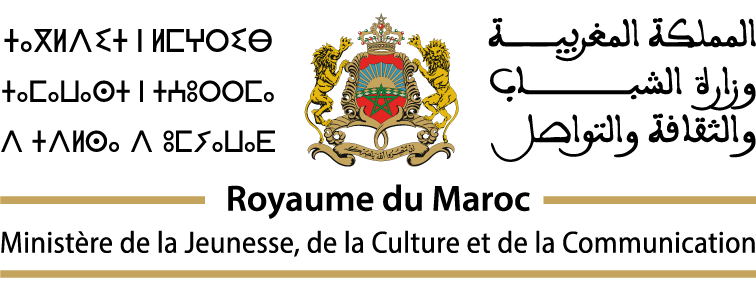
\includegraphics[width=0.8\textwidth]{ministre.png}
		\end{minipage}
		
		\vspace{1.5cm}
		
		{\Large \textbf{École Supérieure de Technologie de Ouarzazate}}\\[0.3cm]
		{\large Filière : Data Engineering}\\[1.5cm]
		
		{\Huge \textbf{Rapport de stage}}\\[1cm]
		
		{\Large
			effectué au sein du Ministère de la Jeunesse, de la Culture et de la Communication
		}\\[1.5cm]
		
		\rule{\textwidth}{0.8pt}\\[0.4cm]
		
		{\LARGE \textbf{
				Conception d’un système décisionnel\\
				pour l’analyse de la billetterie\\
				des monuments historiques
		}}\\[0.4cm]
		
		\rule{\textwidth}{0.8pt}
		
		\vspace{1.5cm}
		
		\begin{flushleft}
			\renewcommand{\arraystretch}{1.5}
			\begin{tabular}{p{6cm} p{8cm}}
				\textbf{Réalisé par :} & OUBLAL Haytam \\
				\textbf{Encadrante pédagogique :} & OUIDRINE Fatima \\
				\textbf{Encadrant professionnel :} & BELHADJ Khalid \\
			\end{tabular}
		\end{flushleft}
		
		\vfill
		
		\begin{center}
			\textbf{Période de stage :}\\
			Du 1 Avril au 30 Mai 2026\\[0.5cm]
			
			\textbf{Année universitaire : 2025--2026}
		\end{center}
		
	\end{titlepage}
	
	% ==================================================
	% PAGE VIDE
	% ==================================================
	
	\newpage
	\thispagestyle{empty}
	\mbox{}
	\newpage
	
	% ==================================================
	% REMERCIEMENTS
	% ==================================================
	
	\chapter*{Remerciements}
	\addcontentsline{toc}{chapter}{Remerciements}
	
	\vspace{1cm}
	
	% À compléter plus tard
	
	\newpage
	
	% ==================================================
	% RESUME
	% ==================================================
	
	\chapter*{Résumé}
	\addcontentsline{toc}{chapter}{Résumé}
	
	\vspace{1cm}
	
	% À compléter plus tard
	
	\newpage
	
	% ==================================================
	% ABSTRACT
	% ==================================================
	
	\chapter*{Abstract}
	\addcontentsline{toc}{chapter}{Abstract}
	
	\vspace{1cm}
	
	% To be completed later
	
	\newpage
	
	% ==================================================
	% TABLE DES MATIERES
	% ==================================================
	
	\tableofcontents
	\newpage
	
	\clearpage
	\pagenumbering{arabic}
	
	% ==================================================
	% TABLE DES FIGURES
	% ==================================================
	
	\listoffigures
	\newpage
	
	% ==================================================
	% INTRODUCTION GENERALE
	% ==================================================
	
\chapter*{Introduction générale}
\addcontentsline{toc}{chapter}{Introduction générale}

Avec le développement des technologies numériques et la transformation digitale, les organisations produisent quotidiennement un volume important de données provenant de différentes sources. Ces données représentent une ressource stratégique permettant d’améliorer le suivi des activités, l’analyse des performances ainsi que la prise de décision.

Dans le domaine culturel et touristique, les systèmes de billetterie des monuments historiques génèrent de nombreuses données liées aux ventes de tickets, aux recettes, à la fréquentation ainsi qu’aux transactions réalisées au niveau des différents sites culturels. Ces informations peuvent fournir des indicateurs importants pour le pilotage et l’évaluation des performances des monuments historiques.

Cependant, ces données sont souvent dispersées dans plusieurs tables et systèmes opérationnels conçus principalement pour la gestion quotidienne et non pour l’analyse décisionnelle. Cette dispersion rend difficile l’exploitation efficace des données et limite la capacité des responsables à obtenir une vision globale et cohérente de l’activité.

Dans ce contexte, les systèmes décisionnels jouent un rôle essentiel. Ils permettent de centraliser, structurer et exploiter les données afin de produire des informations fiables et pertinentes pour l’aide à la décision. Ces systèmes reposent généralement sur un Data Warehouse, alimenté à travers un processus ETL (Extract, Transform, Load), puis exploité via des outils de visualisation et d’analyse.

C’est dans ce cadre que s’inscrit ce projet de stage effectué au sein du Ministère de la Jeunesse, de la Culture et de la Communication, sous le thème :

\begin{center}
	\textbf{\Large Conception d’un système décisionnel pour l’analyse de la billetterie des monuments historiques}
\end{center}

L’objectif principal de ce projet est de concevoir et mettre en place une solution décisionnelle permettant de centraliser les données de billetterie et de recettes, de les transformer à travers un processus ETL, puis de les exploiter dans des tableaux de bord interactifs afin de faciliter l’analyse et la prise de décision.

Pour atteindre cet objectif, plusieurs étapes ont été réalisées. Une première phase d’analyse des données a permis d’identifier les différentes tables utilisées dans le système de gestion, notamment les tables liées aux recettes, aux transactions, aux commandes de billetterie, aux monuments historiques et aux types de revenus.

Ensuite, un modèle décisionnel basé sur un schéma en étoile a été conçu afin d’organiser les données de manière optimisée pour l’analyse multidimensionnelle. Ce modèle comprend plusieurs dimensions telles que les monuments, les types de revenus ainsi que les transactions de billetterie.

Par la suite, un processus ETL a été développé avec Talend Open Studio afin d’extraire les données depuis les sources, nettoyer les incohérences, harmoniser les formats et charger les données préparées dans un environnement exploitable pour l’analyse.

Enfin, les données transformées ont été intégrées dans Power BI afin de réaliser des tableaux de bord interactifs permettant le suivi des recettes, l’analyse des ventes, la comparaison des performances des monuments historiques ainsi que l’étude de l’évolution des transactions dans le temps.

Les principaux outils utilisés dans ce projet sont :

\begin{itemize}
	\item MySQL pour la gestion des données sources ;
	\item Talend Open Studio pour le processus ETL ;
	\item Power BI pour la visualisation et l’analyse des données.
\end{itemize}

Ce rapport est structuré en plusieurs chapitres. Le premier chapitre présente le contexte du projet ainsi que l’analyse des données sources. Le deuxième chapitre est consacré à la conception du système décisionnel et à la modélisation du Data Warehouse. Le troisième chapitre présente l’implémentation du processus ETL et les transformations appliquées aux données. Enfin, le dernier chapitre est dédié à la visualisation des données et à l’analyse des indicateurs de performance réalisés avec Power BI.
% ==================================================
% CHAPITRE 1
% ==================================================

\chapter{Présentation de l’organisme d’accueil}

\section*{Introduction}
\addcontentsline{toc}{section}{Introduction}

Ce chapitre a pour objectif de présenter l’organisme d’accueil dans lequel le stage a été effectué ainsi que le contexte général du projet. Il permet de mieux comprendre l’environnement professionnel dans lequel s’inscrit la réalisation du système décisionnel développé durant ce stage.

Dans un premier temps, ce chapitre présente le Ministère de la Jeunesse, de la Culture et de la Communication, ses principales missions ainsi que son rôle dans la gestion et la valorisation du patrimoine culturel marocain. Ensuite, le service d’affectation est présenté afin de situer le cadre technique et organisationnel du projet.

Enfin, ce chapitre introduit l’environnement de travail et les principaux outils utilisés durant le stage, notamment les technologies liées aux bases de données, au processus ETL et à la Business Intelligence.

% --------------------------------------------------

\section{Présentation du ministère}

\begin{figure}[H]
	\centering
	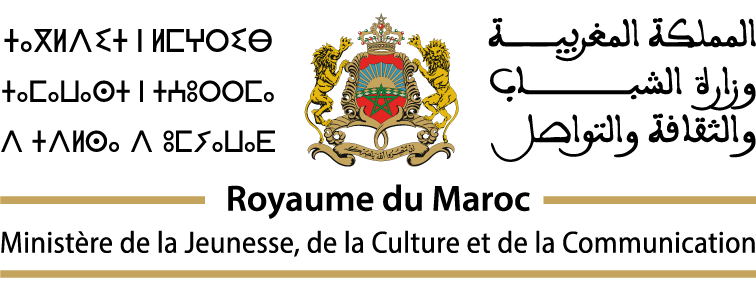
\includegraphics[width=0.45\textwidth]{ministre.png}
	\caption{Logo du Ministère de la Jeunesse, de la Culture et de la Communication}
\end{figure}

Le stage a été réalisé au sein du Ministère de la Jeunesse, de la Culture et de la Communication. Cette institution publique joue un rôle important dans la gestion, la protection et la valorisation du patrimoine culturel marocain.

Le ministère intervient dans plusieurs domaines liés à la culture, à la communication et à la jeunesse. Parmi ses principales missions figurent la gestion des monuments historiques, l’organisation des activités culturelles ainsi que la modernisation des services destinés au public.

Dans ce contexte, les systèmes d’information occupent une place essentielle, notamment pour la gestion des données liées aux activités de billetterie et aux recettes générées par les sites culturels.

% --------------------------------------------------

\section{Service d’affectation}

Le stage s’est déroulé au sein du service informatique du ministère. Ce service est chargé de la gestion des systèmes d’information, du traitement des données ainsi que du suivi des solutions numériques utilisées dans les différents services.

Le projet réalisé dans le cadre de ce stage consiste à concevoir un système décisionnel permettant d’analyser les données de billetterie des monuments historiques afin de produire des indicateurs de performance utiles pour l’aide à la décision.

Ce projet s’inscrit dans une démarche de valorisation des données et d’amélioration de l’exploitation des informations générées par les systèmes de gestion.

% --------------------------------------------------

\section{Missions du ministère}

Le Ministère de la Jeunesse, de la Culture et de la Communication assure plusieurs missions importantes liées à la gestion et à la valorisation du patrimoine culturel marocain.

Parmi ses principales missions, on peut citer :

\begin{itemize}
	\item la protection et la conservation des monuments historiques ;
	\item la promotion des activités culturelles ;
	\item la gestion des sites culturels et touristiques ;
	\item l’amélioration des services destinés au public ;
	\item la modernisation des systèmes d’information et des outils numériques.
\end{itemize}

Le ministère joue également un rôle important dans l’exploitation des données liées aux activités culturelles afin d’améliorer la gestion et le suivi des performances.

% --------------------------------------------------

\section{Environnement technique}

La réalisation de ce projet a nécessité l’utilisation de plusieurs outils et technologies permettant de traiter, transformer et analyser les données.

Les principaux outils utilisés sont :

\begin{itemize}
	\item \textbf{MySQL} pour la gestion des données sources ;
	\item \textbf{Talend Open Studio} pour le développement du processus ETL ;
	\item \textbf{Power BI} pour la modélisation et la visualisation des données ;
	\item \textbf{GitHub} pour le suivi et l’organisation du projet.
\end{itemize}

Ces outils ont permis de mettre en place une solution décisionnelle complète pour l’analyse des données de billetterie et des recettes.

% --------------------------------------------------

\section*{Conclusion}
\addcontentsline{toc}{section}{Conclusion}

Ce chapitre a permis de présenter l’organisme d’accueil ainsi que le contexte général dans lequel le stage a été réalisé. Il a également présenté le service d’affectation, les principales missions du ministère ainsi que l’environnement technique utilisé dans le cadre du projet.

Cette étape constitue une base importante pour comprendre le contexte du projet avant d’aborder l’analyse des données et la conception du système décisionnel.
% ==================================================
% CHAPITRE 2
% ==================================================

\chapter{Analyse des données sources}

\section*{Introduction}
\addcontentsline{toc}{section}{Introduction}

Avant de concevoir un système décisionnel, il est nécessaire de réaliser une analyse détaillée des données sources. Cette étape permet de comprendre la structure de la base de données, d’identifier les tables importantes et de déterminer les relations existantes entre les différentes entités.

Dans le cadre de ce projet, l’analyse des données sources a permis de mieux comprendre le fonctionnement du système de billetterie des monuments historiques. Elle a également permis d’identifier les différentes sources de revenus, notamment les recettes saisies manuellement et les recettes issues du système de billetterie.

Ce chapitre présente donc les principales tables de la base de données, les sources de revenus retenues, les tables de contexte utilisées dans l’analyse ainsi que les relations entre les données. Cette analyse constitue une étape essentielle avant la conception du Data Warehouse et la mise en place du processus ETL.

% --------------------------------------------------

\section{Présentation générale de la base de données}

Les données exploitées dans ce projet proviennent d’une base de données relationnelle utilisée pour la gestion des recettes et de la billetterie des monuments historiques. Cette base contient plusieurs tables permettant de stocker les informations relatives aux monuments, aux régies, aux recettes, aux commandes de billetterie, aux types de tickets et aux transactions financières.

\begin{figure}[H]
	\centering
	\includegraphics[width=0.75\textwidth]{pics/01_liste_tables_base_donnees.png}
	\caption{Liste des tables de la base de données source}
	\label{fig:liste_tables_base}
\end{figure}

La figure \ref{fig:liste_tables_base} présente les principales tables disponibles dans la base de données. Ces tables constituent la source principale utilisée pour la conception du système décisionnel.

\begin{table}[H]
	\centering
	\renewcommand{\arraystretch}{1.3}
	\begin{tabular}{|p{5cm}|p{9cm}|}
		\hline
		\textbf{Table} & \textbf{Rôle dans la base de données} \\
		\hline
		\texttt{places} & Contient les informations relatives aux monuments et sites culturels. \\
		\hline
		\texttt{regies} & Contient les informations relatives aux régies responsables de la gestion des monuments. \\
		\hline
		\texttt{recettes} & Contient les recettes saisies manuellement dans le système. \\
		\hline
		\texttt{revenue\_types} & Contient les différents types de revenus. \\
		\hline
		\texttt{ticketing\_commands} & Contient les commandes générées par le système de billetterie. \\
		\hline
		\texttt{ticketing\_command\_lines} & Contient les détails des commandes de billetterie, notamment les quantités et les montants par type de ticket. \\
		\hline
		\texttt{ticket\_types} & Contient les informations relatives aux types de tickets et à leurs prix. \\
		\hline
		\texttt{ticket\_types\_titles} & Contient les catégories ou intitulés des types de tickets. \\
		\hline
		\texttt{transactions} & Contient des informations relatives aux transactions financières. \\
		\hline
	\end{tabular}
	\caption{Description générale des tables de la base de données}
	\label{tab:description_tables}
\end{table}

Cette présentation globale permet d’avoir une vision claire sur les différentes entités de la base de données. Toutefois, toutes les tables ne seront pas détaillées au même niveau dans ce rapport. L’analyse se concentre principalement sur les tables les plus importantes pour la construction du modèle décisionnel.

% --------------------------------------------------

\section{Identification des principales sources de revenus}

L’analyse de la base de données a montré que les revenus ne sont pas stockés dans une seule table. En effet, les données financières proviennent principalement de deux sources : les recettes saisies manuellement et les recettes issues du système de billetterie.

Cette distinction est importante, car elle évite de considérer la table \texttt{recettes} comme l’unique source de revenus. Une telle hypothèse aurait conduit à une analyse partielle de l’activité réelle des monuments historiques.

% --------------------------------------------------

\subsection{Recettes saisies manuellement}

La table \texttt{recettes} contient les recettes enregistrées manuellement dans le système. Elle comprend notamment le type de revenu, le monument concerné, la date de versement et le montant de la recette.

\begin{figure}[H]
	\centering
	\includegraphics[width=0.9\textwidth]{pics/05_apercu_recettes.png}
	\caption{Aperçu des données de la table \texttt{recettes}}
	\label{fig:apercu_recettes}
\end{figure}

Comme le montre la figure \ref{fig:apercu_recettes}, chaque ligne de la table \texttt{recettes} représente une opération financière associée à un monument et à un type de revenu. Cette table permet donc d’analyser les recettes manuelles selon plusieurs axes, tels que le site, la date ou la nature du revenu.

Les principaux champs utilisés sont :

\begin{itemize}
	\item \texttt{id} : identifiant unique de la recette ;
	\item \texttt{revenue\_type\_id} : identifiant du type de revenu ;
	\item \texttt{place\_id} : identifiant du monument concerné ;
	\item \texttt{date\_versement} : date du versement ;
	\item \texttt{amount} : montant de la recette ;
	\item \texttt{created\_at} : date de création de l’enregistrement.
\end{itemize}

Cette table constitue une source importante pour le système décisionnel, mais elle ne représente pas à elle seule l’ensemble des revenus générés par les monuments.

% --------------------------------------------------

\subsection{Recettes issues du système de billetterie}

Les recettes issues du système de billetterie sont principalement stockées dans les tables \texttt{ticketing\_commands} et \texttt{ticketing\_command\_lines}.

La table \texttt{ticketing\_commands} contient les informations générales relatives aux commandes de billetterie, comme la date de création, le montant total, le statut du paiement, le monument concerné et la référence de transaction.

\begin{figure}[H]
	\centering
	\includegraphics[width=0.9\textwidth]{pics/06_apercu_ticketing_commands.png}
	\caption{Aperçu des commandes de billetterie}
	\label{fig:apercu_ticketing_commands}
\end{figure}

La figure \ref{fig:apercu_ticketing_commands} montre que chaque commande de billetterie contient un montant total, un statut et un lien avec un monument à travers le champ \texttt{place\_id}. Cette table permet donc de suivre les ventes globales issues du système de billetterie.

La table \texttt{ticketing\_command\_lines} contient quant à elle les détails des commandes, notamment le type de ticket, la quantité et le montant de chaque ligne de commande.

\begin{figure}[H]
	\centering
	\includegraphics[width=0.9\textwidth]{pics/07_apercu_ticketing_command_lines.png}
	\caption{Aperçu des lignes de commandes de billetterie}
	\label{fig:apercu_ticketing_command_lines}
\end{figure}

La figure \ref{fig:apercu_ticketing_command_lines} permet de comprendre le niveau de détail du système de billetterie. Elle montre que chaque commande peut contenir une ou plusieurs lignes, chacune associée à un type de ticket, une quantité et un montant.

Ainsi, les tables \texttt{ticketing\_commands} et \texttt{ticketing\_command\_lines} sont essentielles pour analyser les ventes issues du système de billetterie.

% --------------------------------------------------

\section{Tables de contexte utilisées dans l’analyse}

En plus des tables contenant les mesures financières, certaines tables jouent un rôle de contexte. Elles permettent d’enrichir l’analyse en ajoutant des informations sur les monuments, les régies, les types de revenus ou encore les types de tickets.

% --------------------------------------------------

\subsection{Table \texttt{places}}

La table \texttt{places} contient les informations relatives aux monuments et sites culturels. Elle permet d’identifier le nom du monument, la régie associée, la ville et l’existence éventuelle d’un système de billetterie.

\begin{figure}[H]
	\centering
	\includegraphics[width=0.9\textwidth]{pics/08_apercu_places.png}
	\caption{Aperçu des données de la table \texttt{places}}
	\label{fig:apercu_places}
\end{figure}

Le champ \texttt{is\_ticketing} est particulièrement important, car il permet de distinguer les sites qui disposent d’un système de billetterie de ceux qui n’en disposent pas. Cette information peut être utilisée dans l’analyse décisionnelle pour comparer les revenus selon le mode de gestion des sites.

% --------------------------------------------------

\subsection{Table \texttt{revenue\_types}}

La table \texttt{revenue\_types} contient les différents types de revenus enregistrés dans le système. Elle permet de classifier les recettes selon leur nature.

\begin{figure}[H]
	\centering
	\includegraphics[width=0.85\textwidth]{pics/09_apercu_revenue_types.png}
	\caption{Aperçu des types de revenus}
	\label{fig:apercu_revenue_types}
\end{figure}

Cette table est utilisée comme une dimension dans le modèle décisionnel, car elle permet d’analyser les recettes selon leur type, par exemple les droits de visite, les locations ou les inscriptions.

% --------------------------------------------------

\subsection{Autres tables de contexte}

D’autres tables complètent l’analyse et peuvent être utilisées selon les besoins du modèle décisionnel.

La table \texttt{regies} permet de relier les monuments aux entités responsables de leur gestion. Elle est utile pour analyser les recettes par régie et comparer les performances des différentes structures de gestion.

La table \texttt{ticket\_types} contient les types de tickets ainsi que leurs prix. Elle est utilisée pour analyser les ventes selon les catégories de tickets.

La table \texttt{ticket\_types\_titles} permet de décrire les intitulés des types de tickets et peut contenir des informations supplémentaires telles que le caractère groupé ou étranger du ticket.

Enfin, la table \texttt{transactions} contient des données relatives aux transactions financières, notamment les montants, les méthodes de paiement, les statuts et les dates de paiement. Elle peut enrichir l’analyse des paiements lorsque ces informations sont nécessaires.

% --------------------------------------------------

\section{Analyse des relations entre les tables}

Après l’identification des principales tables, il est nécessaire d’analyser les relations entre elles. Cette étape permet de comprendre comment les données peuvent être reliées afin de construire un modèle décisionnel cohérent.

% --------------------------------------------------

\subsection{Relation entre les recettes, les monuments et les types de revenus}

La première relation importante concerne la table \texttt{recettes}. Celle-ci est liée à la table \texttt{places} à travers le champ \texttt{place\_id}, ce qui permet d’associer chaque recette à un monument.

Elle est également liée à la table \texttt{revenue\_types} à travers le champ \texttt{revenue\_type\_id}, ce qui permet de connaître la nature de chaque recette.

\begin{figure}[H]
	\centering
	\includegraphics[width=0.95\textwidth]{pics/11_jointure_recettes_places_revenu_types.png}
	\caption{Jointure entre les recettes, les monuments et les types de revenus}
	\label{fig:jointure_recettes}
\end{figure}

La figure \ref{fig:jointure_recettes} illustre la relation entre les recettes, les monuments et les types de revenus. Cette jointure permet de préparer une analyse des recettes par site, par type de revenu et par période.

% --------------------------------------------------

\subsection{Relation entre les commandes de billetterie et leurs détails}

La deuxième relation importante concerne le système de billetterie. La table \texttt{ticketing\_commands} contient les commandes globales, tandis que la table \texttt{ticketing\_command\_lines} contient les détails de chaque commande.

La relation entre ces deux tables se fait à travers le champ \texttt{ticketing\_command\_id}. La table \texttt{ticketing\_commands} est également reliée à la table \texttt{places} à travers le champ \texttt{place\_id}.

\begin{figure}[H]
	\centering
	\includegraphics[width=0.95\textwidth]{pics/12_jointure_ticketing_systeme.png}
	\caption{Jointure entre les commandes de billetterie, les lignes de commandes et les monuments}
	\label{fig:jointure_ticketing}
\end{figure}

La figure \ref{fig:jointure_ticketing} montre que les ventes issues du système de billetterie peuvent être analysées selon le monument, la date, le montant, le statut de la commande et la quantité de tickets vendus.

% --------------------------------------------------

\section{Qualité et limites des données}

L’analyse des données sources a également permis de relever certaines limites qui doivent être prises en compte avant l’intégration dans le système décisionnel.

Les principales limites observées sont :

\begin{itemize}
	\item la dispersion des données financières dans plusieurs tables ;
	\item la présence possible de valeurs manquantes dans certaines colonnes ;
	\item l’existence de champs textuels nécessitant un nettoyage ;
	\item la présence de données stockées sous des formats techniques, comme le format JSON dans certains noms de monuments ;
	\item la nécessité d’harmoniser les formats de dates et de montants.
\end{itemize}

Ces limites justifient la mise en place d’un processus ETL afin de nettoyer, transformer et structurer les données avant leur exploitation dans Power BI.

% --------------------------------------------------

\section*{Conclusion}
\addcontentsline{toc}{section}{Conclusion}

Ce chapitre a permis de présenter et d’analyser les données sources utilisées dans le projet. L’étude de la base de données a montré que les revenus des monuments historiques proviennent principalement de deux sources : les recettes saisies manuellement et les commandes issues du système de billetterie.

L’analyse a également permis d’identifier les tables de contexte nécessaires à l’interprétation des données, notamment les tables \texttt{places}, \texttt{regies}, \texttt{revenue\_types}, \texttt{ticket\_types} et \texttt{ticket\_types\_titles}.

Enfin, les relations entre les tables ont été étudiées afin de préparer la conception du modèle décisionnel. Cette étape constitue une base essentielle pour la construction du Data Warehouse et la mise en place du processus ETL.
% ==================================================
% CHAPITRE 3
% ==================================================

\chapter{Conception du système décisionnel et processus ETL}

\section*{Introduction}
\addcontentsline{toc}{section}{Introduction}

Après l’analyse des données sources, cette étape consiste à présenter la conception générale du système décisionnel ainsi que le processus ETL adopté pour préparer les données à l’analyse.

Ce chapitre a pour objectif d’expliquer le principe d’un système décisionnel, de présenter le rôle du processus ETL, puis de décrire les données sélectionnées pour la construction du modèle analytique. Il présente également le schéma décisionnel réalisé dans Power BI, en mettant en évidence les tables de faits, les tables de dimensions et les principales relations entre les tables.

Cette étape constitue une transition entre l’analyse des données sources et l’implémentation pratique des transformations avec Talend Open Studio.

% --------------------------------------------------

\section{Notion de système décisionnel}

Un système décisionnel est un ensemble de méthodes, d’outils et de processus permettant de transformer des données brutes en informations utiles pour la prise de décision. Contrairement aux systèmes opérationnels, qui sont principalement utilisés pour gérer les activités quotidiennes, un système décisionnel est orienté vers l’analyse, le suivi des performances et l’aide au pilotage.

Dans le cadre de ce projet, le système décisionnel permet d’exploiter les données liées à la billetterie et aux recettes des monuments historiques afin de produire des indicateurs fiables. Ces indicateurs peuvent aider les responsables à suivre l’évolution des recettes, comparer les performances des monuments et identifier les périodes ou les sites les plus importants.

Un système décisionnel repose généralement sur plusieurs composants :

\begin{itemize}
	\item les sources de données, qui contiennent les données opérationnelles ;
	\item le processus ETL, qui permet d’extraire, de transformer et de charger les données ;
	\item le Data Warehouse, qui permet de stocker les données préparées sous une forme structurée ;
	\item les outils de visualisation, qui permettent de créer des tableaux de bord et des indicateurs de performance.
\end{itemize}

Ainsi, la mise en place d’un système décisionnel permet de passer d’une base de données opérationnelle complexe à une information claire, organisée et exploitable pour l’analyse.

% --------------------------------------------------

\section{Présentation du processus ETL}

Le processus ETL, abréviation de \textit{Extract, Transform, Load}, représente une étape essentielle dans la mise en place d’un système décisionnel. Il permet de préparer les données avant leur intégration dans un Data Warehouse ou dans un outil d’analyse comme Power BI.

Ce processus se déroule en trois phases principales :

\begin{itemize}
	\item \textbf{Extraction} : cette phase consiste à récupérer les données depuis les sources disponibles, comme une base de données MySQL ou des fichiers CSV.
	\item \textbf{Transformation} : cette phase consiste à nettoyer les données, corriger les formats, traiter les valeurs manquantes et préparer les colonnes nécessaires à l’analyse.
	\item \textbf{Chargement} : cette phase consiste à charger les données transformées dans un espace structuré, afin de les exploiter dans le modèle décisionnel.
\end{itemize}

\begin{figure}[H]
	\centering
	\includegraphics[width=0.9\textwidth]{pics/7_architecture_decisionnelle.png}
	\caption{Principe général du processus ETL}
	\label{fig:processus_etl}
\end{figure}

La figure \ref{fig:processus_etl} illustre le fonctionnement général d’un processus ETL. Les données sont d’abord extraites depuis les sources, puis transformées afin d’améliorer leur qualité. Elles sont ensuite chargées dans un Data Warehouse, avant d’être utilisées pour l’analyse et la visualisation.

Dans ce projet, l’outil Talend Open Studio a été choisi pour la mise en œuvre du processus ETL, tandis que Power BI a été utilisé pour la modélisation et l’analyse des données.

% --------------------------------------------------

\section{Extraction des données sources}

La première étape pratique du processus ETL consiste à extraire les données depuis la base de données source. Dans ce projet, les données ont été exportées depuis MySQL sous forme de fichiers CSV afin de faciliter leur traitement dans les outils d’analyse.

Cette extraction permet de séparer les données utiles du système opérationnel et de les préparer pour les étapes suivantes. Les fichiers CSV obtenus constituent une base de travail pour la transformation des données et leur intégration dans le modèle décisionnel.

Les tables sélectionnées pour l’extraction sont celles qui participent directement à l’analyse des recettes et de la billetterie. Le choix de ces tables repose sur leur rôle dans le système source, leur contenu analytique et leur relation avec les objectifs du projet.

% --------------------------------------------------

\subsection{Tables sélectionnées}

Les tables retenues pour ce projet sont les suivantes :

\begin{itemize}
	\item \texttt{recettes} : elle contient les recettes saisies manuellement dans le système.
	\item \texttt{ticketing\_commands} : elle contient les commandes globales issues du système de billetterie.
	\item \texttt{ticketing\_command\_line} : elle contient les lignes détaillées des commandes de billetterie, notamment les quantités et les montants.
	\item \texttt{places} : elle contient les informations relatives aux monuments et sites culturels.
	\item \texttt{regies} : elle contient les informations relatives aux régies responsables de la gestion des monuments.
	\item \texttt{revenue\_types} : elle contient les types de revenus associés aux recettes.
	\item \texttt{ticket\_types} : elle contient les types de tickets et leurs prix.
	\item \texttt{tickets\_type\_titles} : elle contient les intitulés et catégories des types de tickets.
\end{itemize}

Ces tables permettent de couvrir les deux principales sources de revenus identifiées dans l’analyse des données : les recettes saisies manuellement et les recettes générées par le système de billetterie.

% --------------------------------------------------

\section{Modélisation du schéma décisionnel}

Après l’extraction des tables nécessaires, une modélisation décisionnelle a été réalisée afin d’organiser les données de manière adaptée à l’analyse. Le modèle adopté repose sur une logique de schéma en étoile étendu, car il intègre plusieurs tables de faits et plusieurs dimensions.

Ce choix se justifie par la structure de la base source. En effet, les données financières ne sont pas stockées dans une seule table. La table \texttt{recettes} représente les recettes saisies manuellement, tandis que les ventes de billetterie sont représentées par les tables \texttt{ticketing\_commands} et \texttt{ticketing\_command\_line}.

% --------------------------------------------------

\subsection{Tables de faits}

Dans ce modèle, deux tables jouent le rôle de tables de faits principales.

La première table de faits est la table \texttt{recettes}. Elle contient les mesures financières liées aux recettes manuelles, notamment le montant de la recette, la date de versement, le monument concerné et le type de revenu.

La deuxième table de faits est la table \texttt{ticketing\_command\_line}. Elle contient les détails des ventes de tickets, notamment la quantité vendue, le montant de la ligne et le type de ticket. Cette table représente le niveau détaillé des transactions de billetterie.

La table \texttt{ticketing\_commands} joue un rôle complémentaire, car elle contient les informations générales de la commande, comme la date, le statut, le montant total et le monument concerné.

% --------------------------------------------------

\subsection{Tables de dimensions}

Les tables de dimensions permettent d’enrichir les tables de faits en ajoutant des axes d’analyse.

Dans ce modèle, les principales dimensions sont :

\begin{itemize}
	\item \texttt{places} : permet d’analyser les données par monument ou site culturel.
	\item \texttt{regies} : permet d’analyser les performances par régie.
	\item \texttt{revenue\_types} : permet d’analyser les recettes selon leur type.
	\item \texttt{ticket\_types} : permet d’analyser les ventes selon le type de ticket.
	\item \texttt{tickets\_type\_titles} : permet d’ajouter une description plus détaillée des catégories de tickets.
\end{itemize}

La dimension \texttt{regies} est liée indirectement aux recettes à travers la table \texttt{places}. Cette relation permet d’analyser les recettes par régie sans créer de redondance inutile dans les tables de faits.

% --------------------------------------------------

\subsection{Schéma décisionnel réalisé dans Power BI}

Le modèle relationnel a été construit dans Power BI afin de visualiser les relations entre les tables et de préparer les futures analyses.

\begin{figure}[H]
	\centering
	
\includegraphics[width=0.95\textwidth]{pics/14_schema_etoile_powerbi.png}
	\caption{Schéma décisionnel réalisé dans Power BI}
	\label{fig:schema_etoile_powerbi}
\end{figure}

La figure \ref{fig:schema_etoile_powerbi} présente le schéma décisionnel réalisé. Ce modèle met en évidence les relations entre les tables de faits et les tables de dimensions. Il permet d’analyser les données selon plusieurs axes, notamment les monuments, les régies, les types de revenus, les types de tickets et les dates de transaction.

Les principales relations du modèle sont les suivantes :

\begin{itemize}
	\item \texttt{recettes.place\_id} est liée à \texttt{places.id}.
	\item \texttt{recettes.revenue\_type\_id} est liée à \texttt{revenue\_types.id}.
	\item \texttt{places.regie\_id} est liée à \texttt{regies.id}.
	\item \texttt{ticketing\_commands.place\_id} est liée à \texttt{places.id}.
	\item \texttt{ticketing\_command\_line.ticketing\_command\_id} est liée à \texttt{ticketing\_commands.id}.
	\item \texttt{ticketing\_command\_line.ticket\_type\_id} est liée à \texttt{ticket\_types.id}.
	\item \texttt{ticket\_types.ticket\_types\_title\_id} est liée à \texttt{tickets\_type\_titles.id}.
\end{itemize}

Ce modèle permet d’éviter une analyse limitée à une seule table et offre une vision plus complète des revenus générés par les monuments historiques.

% --------------------------------------------------
\section{Transformation de la table \texttt{places}}

Après l’extraction de la table \texttt{places} depuis la base de données source, une étape de transformation a été réalisée à l’aide de Talend Open Studio afin de préparer les données pour leur intégration dans le système décisionnel.

La table \texttt{places} contient les informations relatives aux espaces culturels et monuments historiques. Cependant, les données extraites présentaient plusieurs problèmes :
\begin{itemize}
	\item les valeurs de la colonne \texttt{title} étaient stockées sous forme de chaînes JSON ;
	\item certains caractères spéciaux étaient mal encodés ;
	\item plusieurs valeurs étaient nulles ou incomplètes ;
	\item les données n’étaient pas directement exploitables dans Power BI.
\end{itemize}

La Figure~\ref{fig:places_brut} présente un aperçu des données avant transformation. On remarque que les titres contiennent une structure JSON ainsi que des caractères spéciaux encodés, ce qui complique leur exploitation dans les outils d’analyse décisionnelle.

\begin{figure}[H]
	\centering
	\includegraphics[width=1\textwidth]{pics/15_donnees_brutes_places_avant_transformation.png}
	\caption{Données brutes de la table \texttt{places} avant transformation}
	\label{fig:places_brut}
\end{figure}

Afin de corriger ces problèmes, un flux ETL a été développé avec Talend Open Studio. Ce flux permet :
\begin{itemize}
	\item l’extraction des données depuis le fichier CSV source ;
	\item le nettoyage des données ;
	\item la suppression des structures JSON inutiles ;
	\item la correction des problèmes d’encodage ;
	\item la gestion des valeurs manquantes ;
	\item la génération d’un nouveau fichier propre et exploitable.
\end{itemize}

Le workflow ETL utilisé est composé principalement des composants suivants :
\begin{itemize}
	\item \texttt{tFileInputDelimited} pour lire le fichier CSV source ;
	\item \texttt{tMap} pour effectuer les transformations ;
	\item \texttt{tFileOutputDelimited} pour générer le fichier nettoyé.
\end{itemize}

La Figure~\ref{fig:tmap_places} présente la configuration des transformations réalisées dans le composant \texttt{tMap}.

\begin{figure}[H]
	\centering
	\includegraphics[width=1\textwidth]{pics/17_transformation_tmap_places.png}
	\caption{Transformation des données dans le composant \texttt{tMap}}
	\label{fig:tmap_places}
\end{figure}

Plusieurs traitements ont été appliqués afin d’obtenir des données homogènes et exploitables :
\begin{itemize}
	\item suppression des balises JSON ;
	\item suppression des caractères inutiles ;
	\item remplacement des caractères spéciaux encodés ;
	\item nettoyage des espaces inutiles ;
	\item remplacement de certaines valeurs nulles.
\end{itemize}

L’expression suivante a été utilisée dans le composant \texttt{tMap} afin de nettoyer la colonne \texttt{title} :

\begin{lstlisting}[language=Java, caption={Expression de nettoyage appliquee dans le composant tMap}]
	row1.title == null ? "" : 
	row1.title.replace("{\"fr\":\"", "")
		.replace("{\"ar\":\"", "")
			.replace("{\"en\":\"", "")
				.replace("\"", "")
				.replace("}", "")
			.replace("\\u00e9", "e")
			.replace("\\u00e8", "e")
			.replace("\\u00ea", "e")
			.replace("\\u00e0", "a")
			.replace("\\u00e2", "a")
			.replace("\\u00f4", "o")
			.replace("\\u00ee", "i")
			.replace("\\u00f9", "u")
			.replace("\\u00e7", "c")
			.trim()
		\end{lstlisting}
		
		Après la configuration des composants ETL, le job Talend a été exécuté avec succès afin de produire un nouveau fichier contenant les données nettoyées.
		
		\begin{figure}[H]
			\centering
			\includegraphics[width=0.9\textwidth]{pics/18_execution_job_places_success.png}
			\caption{Exécution réussie du job ETL de la table \texttt{places}}
			\label{fig:execution_places}
		\end{figure}
		
		Le résultat final obtenu après transformation est présenté dans la Figure~\ref{fig:places_clean}. Les données sont désormais structurées, nettoyées et prêtes à être intégrées dans le Data Warehouse ainsi qu’exploitées dans Power BI.
		
		\begin{figure}[H]
			\centering
			\includegraphics[width=1\textwidth]{pics/19_resultat_places_out.png}
			\caption{Résultat final de la transformation de la table \texttt{places}}
			\label{fig:places_clean}
		\end{figure}
		\section{Transformation de la table \texttt{regies}}
		
		Après la transformation de la table \texttt{places}, une nouvelle étape ETL a été réalisée sur la table \texttt{regies}. Cette table contient les informations relatives aux régies responsables de la gestion des différents espaces culturels.
		
		Les données extraites contenaient certaines valeurs manquantes ainsi que des espaces inutiles dans certaines colonnes textuelles. Une opération de nettoyage a donc été effectuée afin de garantir la qualité et la cohérence des données avant leur intégration dans le système décisionnel.
		
		La Figure~\ref{fig:regies_brut} présente un aperçu des données avant transformation.
		
		\begin{figure}[H]
			\centering
			\includegraphics[width=1\textwidth]{pics/20_donnees_brutes_regies_avant_transformation.png}
			\caption{Données brutes de la table \texttt{regies}}
			\label{fig:regies_brut}
		\end{figure}
		
		Le processus ETL développé avec Talend Open Studio a permis d’effectuer plusieurs opérations de nettoyage :
		\begin{itemize}
			\item suppression des espaces inutiles dans les colonnes textuelles ;
			\item gestion des valeurs nulles ;
			\item homogénéisation des formats des données ;
			\item préparation des données pour leur intégration dans le Data Warehouse.
		\end{itemize}
		
		La transformation des données a été réalisée dans le composant \texttt{tMap}, comme illustré dans la Figure~\ref{fig:tmap_regies}.
		
		\begin{figure}[H]
			\centering
			\includegraphics[width=1\textwidth]{pics/20_transformation_tmap_regies.png}
			\caption{Transformation des données de la table \texttt{regies} avec \texttt{tMap}}
			\label{fig:tmap_regies}
		\end{figure}
		
		Les valeurs manquantes des colonnes \texttt{city\_id} et \texttt{user\_id} ont été remplacées par la valeur \texttt{0} afin d’éviter les erreurs de chargement et garantir l’intégrité des données lors de l’intégration dans le système décisionnel.
		
		Les expressions suivantes ont été utilisées dans le composant \texttt{tMap} :
		
		\begin{lstlisting}[language=Java, caption={Expressions de transformation appliquees dans le composant tMap}]
			row1.title == null ? "" : row1.title.trim()
			
			row1.code == null ? "" : row1.code.trim()
			
			row1.city_id == null || row1.city_id.trim().equals("") ? "0" : row1.city_id
			
			row1.user_id == null || row1.user_id.trim().equals("") ? "0" : row1.user_id
		\end{lstlisting}
		
		Après la configuration du flux ETL, le job Talend a été exécuté avec succès afin de générer un nouveau fichier contenant les données nettoyées.
		
		\begin{figure}[H]
			\centering
			\includegraphics[width=0.9\textwidth]{pics/22_execution_job_regies_success.png}
			\caption{Exécution réussie du job ETL de la table \texttt{regies}}
			\label{fig:execution_regies}
		\end{figure}
		
		La Figure~\ref{fig:regies_clean} présente le résultat final obtenu après transformation. Les données sont désormais nettoyées, cohérentes et prêtes à être utilisées dans le modèle décisionnel.
		
		\begin{figure}[H]
			\centering
			\includegraphics[width=1\textwidth]{pics/23_resultat_regies_out.png}
			\caption{Résultat final de la transformation de la table \texttt{regies}}
			\label{fig:regies_clean}
		\end{figure}
		\subsection{Transformation de la table \texttt{revenue\_types}}
		
		La table \texttt{revenue\_types} contient les différents types de revenus liés aux activités culturelles et aux monuments historiques. Cette table joue un rôle important dans le système décisionnel, car elle permet de classifier les recettes selon leur nature.
		
		Avant la transformation, certaines anomalies ont été observées dans les données sources, notamment des problèmes d’encodage des caractères spéciaux ainsi que des valeurs manquantes dans la colonne \texttt{revenue\_category\_id}. La Figure~\ref{fig:revenue_types_brute} présente un aperçu des données brutes avant traitement.
		
		\begin{figure}[H]
			\centering
			\includegraphics[width=1\textwidth]{pics/20_table_revenue_types_brute.png}
			\caption{Aperçu de la table \texttt{revenue\_types} avant transformation}
			\label{fig:revenue_types_brute}
		\end{figure}
		
		Le processus ETL a été réalisé dans Talend à l’aide des composants \texttt{tFileInputDelimited}, \texttt{tMap} et \texttt{tFileOutputDelimited}. Une transformation a été appliquée sur la colonne \texttt{title} afin de supprimer les espaces inutiles et normaliser les valeurs textuelles.
		
		Les principales transformations réalisées sont les suivantes :
		
		\begin{itemize}
			\item Suppression des espaces inutiles avec la fonction \texttt{trim()} ;
			\item Correction des problèmes d’encodage des caractères spéciaux ;
			\item Conservation des identifiants d’origine sans modification ;
			\item Remplacement des valeurs manquantes de \texttt{revenue\_category\_id} par la valeur \texttt{0} ;
			\item Génération d’un fichier CSV nettoyé et structuré pour l’intégration dans Power BI.
		\end{itemize}
		
		La Figure~\ref{fig:tmap_revenue_types} illustre les transformations réalisées dans le composant \texttt{tMap}.
		
		\begin{figure}[H]
			\centering
			\includegraphics[width=1\textwidth]{pics/21_transformation_tmap_revenue_types.png}
			\caption{Transformation des données dans le composant \texttt{tMap}}
			\label{fig:tmap_revenue_types}
		\end{figure}
		
		Après l’exécution du job ETL, un fichier nettoyé et structuré a été généré avec succès. La Figure~\ref{fig:execution_revenue_types} présente l’exécution du job dans Talend.
		
		\begin{figure}[H]
			\centering
			\includegraphics[width=0.9\textwidth]{pics/22_execution_job_revenue_types.png}
			\caption{Exécution du job ETL de la table \texttt{revenue\_types}}
			\label{fig:execution_revenue_types}
		\end{figure}
		
		Le résultat final après transformation est illustré dans la Figure~\ref{fig:resultat_revenue_types}.
		
		\begin{figure}[H]
			\centering
			\includegraphics[width=1\textwidth]{pics/23_resultat_revenue_types_out.png}
			\caption{Résultat final de la transformation de la table \texttt{revenue\_types}}
			\label{fig:resultat_revenue_types}
		\end{figure}
		
		Cette transformation a permis d’obtenir des données propres, homogènes et exploitables dans le système décisionnel et les tableaux de bord Power BI.
		\subsection{Transformation de la table \texttt{recettes}}
		
		La table \texttt{recettes} représente l’une des principales tables de faits du modèle décisionnel. Elle contient les informations relatives aux recettes saisies manuellement, notamment l’identifiant de la recette, le type de revenu, le monument concerné, la date de versement, le montant et la date de création.
		
		Cette table est importante dans le projet, car elle permet d’analyser les recettes selon plusieurs axes : le monument, le type de revenu et la période. Avant son intégration dans le système décisionnel, une étape de transformation a été réalisée afin de garantir la cohérence des données et d’éviter les erreurs lors du chargement dans Power BI.
		
		La Figure~\ref{fig:recettes_brute} présente un aperçu de la table \texttt{recettes} avant transformation.
		
		\begin{figure}[H]
			\centering
			\includegraphics[width=1\textwidth]{pics/24_table_recettes_brute.png}
			\caption{Aperçu de la table \texttt{recettes} avant transformation}
			\label{fig:recettes_brute}
		\end{figure}
		
		Le traitement ETL de cette table a été réalisé avec Talend Open Studio à l’aide des composants \texttt{tFileInputDelimited}, \texttt{tMap} et \texttt{tFileOutputDelimited}. Dans cette transformation, les colonnes ont été traitées sous forme de chaînes de caractères afin d’éviter les erreurs de conversion liées aux valeurs manquantes ou aux formats non homogènes.
		
		Les principales transformations réalisées sont les suivantes :
		
		\begin{itemize}
			\item conservation de l’identifiant de la recette sans modification ;
			\item remplacement des valeurs manquantes de \texttt{revenue\_type\_id} par \texttt{0} ;
			\item remplacement des valeurs manquantes de \texttt{place\_id} par \texttt{0} ;
			\item nettoyage des dates avec la fonction \texttt{trim()} ;
			\item remplacement des montants vides par \texttt{0} ;
			\item conservation de la date de création après nettoyage des espaces inutiles.
		\end{itemize}
		
		La Figure~\ref{fig:tmap_recettes} illustre la configuration des transformations réalisées dans le composant \texttt{tMap}.
		
		\begin{figure}[H]
			\centering
			\includegraphics[width=1\textwidth]{pics/25_transformation_tmap_recettes.png}
			\caption{Transformation des données de la table \texttt{recettes} dans \texttt{tMap}}
			\label{fig:tmap_recettes}
		\end{figure}
		
		Les expressions utilisées dans le composant \texttt{tMap} sont les suivantes :
		
	\begin{lstlisting}[language=Java,breaklines=true,basicstyle=\ttfamily\small]
		
		row1.id
		
		row1.revenue_type_id == null ||
		row1.revenue_type_id.trim().equals("")
		? "0"
		: row1.revenue_type_id
		
		row1.place_id == null ||
		row1.place_id.trim().equals("")
		? "0"
		: row1.place_id
		
		row1.date_versement == null
		? ""
		: row1.date_versement.trim()
		
		row1.amount == null ||
		row1.amount.trim().equals("")
		? "0"
		: row1.amount
		
		row1.created_at == null
		? ""
		: row1.created_at.trim()
		
	\end{lstlisting}
		
		Après la configuration du flux ETL, le job Talend a été exécuté avec succès afin de générer un fichier propre et structuré.
		
		\begin{figure}[H]
			\centering
			\includegraphics[width=0.9\textwidth]{pics/26_execution_job_recettes.png}
			\caption{Exécution du job ETL de la table \texttt{recettes}}
			\label{fig:execution_recettes}
		\end{figure}
		
		Le résultat final obtenu après transformation est présenté dans la Figure~\ref{fig:resultat_recettes}. Les données sont désormais prêtes à être intégrées dans le Data Warehouse et exploitées dans Power BI pour la création des indicateurs de performance.
		
		\begin{figure}[H]
			\centering
			\includegraphics[width=1\textwidth]{pics/27_resultat_recettes_out.png}
			\caption{Résultat final de la transformation de la table \texttt{recettes}}
			\label{fig:resultat_recettes}
		\end{figure}
		\subsection{Transformation de la table \texttt{ticketing\_commands}}
		
		La table \texttt{ticketing\_commands} représente les commandes issues du système de billetterie. Elle contient des informations importantes telles que l’identifiant de la commande, l’utilisateur, les dates de création et de mise à jour, la référence, le montant, le statut de paiement, le monument concerné ainsi que la référence de transaction.
		
		Cette table joue un rôle essentiel dans l’analyse des ventes de billetterie, car elle permet de relier les commandes aux monuments à travers la colonne \texttt{place\_id}. Avant son exploitation dans Power BI, une transformation a été réalisée afin de traiter les valeurs manquantes et d’homogénéiser les champs textuels.
		
		La Figure~\ref{fig:ticketing_commands_brute} présente un aperçu de la table \texttt{ticketing\_commands} avant transformation.
		
		\begin{figure}[H]
			\centering
			\includegraphics[width=1\textwidth]{pics/28_table_ticketing_commands_brute.png}
			\caption{Aperçu de la table \texttt{ticketing\_commands} avant transformation}
			\label{fig:ticketing_commands_brute}
		\end{figure}
		
		Les principales transformations réalisées sont les suivantes :
		
		\begin{itemize}
			\item conservation des identifiants d’origine ;
			\item nettoyage des champs de dates avec la fonction \texttt{trim()} ;
			\item remplacement des montants manquants par la valeur \texttt{0} ;
			\item nettoyage du statut de paiement ;
			\item remplacement des références de transaction manquantes par une chaîne vide ;
			\item génération d’un fichier CSV propre et exploitable dans Power BI.
		\end{itemize}
		
		La Figure~\ref{fig:tmap_ticketing_commands} illustre les transformations réalisées dans le composant \texttt{tMap}.
		
		\begin{figure}[H]
			\centering
			\includegraphics[width=1\textwidth]{pics/29_transformation_tmap_ticketing_commands.png}
			\caption{Transformation des données de la table \texttt{ticketing\_commands} dans \texttt{tMap}}
			\label{fig:tmap_ticketing_commands}
		\end{figure}
		
		Les expressions utilisées dans le composant \texttt{tMap} sont les suivantes :
		
		\begin{lstlisting}[language=Java,breaklines=true,basicstyle=\ttfamily\small]
			row1.id
			
			row1.user_id
			
			row1.created_at == null
			? ""
			: row1.created_at.trim()
			
			row1.updated_at == null
			? ""
			: row1.updated_at.trim()
			
			row1.reference == null
			? ""
			: row1.reference.trim()
			
			row1.amount == null ||
			row1.amount.trim().equals("") ||
			row1.amount.trim().equals("NULL")
			? "0"
			: row1.amount
			
			row1.status == null
			? ""
			: row1.status.trim()
			
			row1.place_id == null ||
			row1.place_id.trim().equals("") ||
			row1.place_id.trim().equals("NULL")
			? "0"
			: row1.place_id
			
			row1.reference_transaction == null ||
			row1.reference_transaction.trim().equals("NULL")
			? ""
			: row1.reference_transaction.trim()
		\end{lstlisting}
		
		Après l’exécution du job ETL, un fichier nettoyé a été généré. La Figure~\ref{fig:execution_ticketing_commands} présente l’exécution réussie du job Talend.
		
		\begin{figure}[H]
			\centering
			\includegraphics[width=0.9\textwidth]{pics/30_execution_job_ticketing_commands.png}
			\caption{Exécution du job ETL de la table \texttt{ticketing\_commands}}
			\label{fig:execution_ticketing_commands}
		\end{figure}
		
		Le résultat final obtenu après transformation est présenté dans la Figure~\ref{fig:resultat_ticketing_commands}. Les données sont désormais structurées et prêtes à être utilisées dans le modèle décisionnel.
		
		\begin{figure}[H]
			\centering
			\includegraphics[width=1\textwidth]{pics/31_resultat_ticketing_commands_out.png}
			\caption{Résultat final de la transformation de la table \texttt{ticketing\_commands}}
			\label{fig:resultat_ticketing_commands}
		\end{figure}
		\subsection{Transformation de la table \texttt{ticketing\_command\_line}}
		
		La table \texttt{ticketing\_command\_line} contient les détails des lignes de commande associées au système de billetterie. Elle représente les ventes détaillées des tickets et contient notamment les identifiants des commandes, les types de tickets, les quantités vendues, les montants ainsi que les réductions appliquées.
		
		Cette table joue un rôle important dans le système décisionnel, car elle permet d’analyser précisément les ventes de tickets selon plusieurs dimensions telles que le type de ticket, la quantité vendue et les revenus générés.
		
		La Figure~\ref{fig:ticketing_command_line_brute} présente un aperçu de la table avant transformation.
		
		\begin{figure}[H]
			\centering
			\includegraphics[width=1\textwidth]{pics/32_table_ticketing_command_line_brute.png}
			\caption{Aperçu de la table \texttt{ticketing\_command\_line} avant transformation}
			\label{fig:ticketing_command_line_brute}
		\end{figure}
		
		Le processus ETL a été réalisé avec Talend Open Studio à l’aide des composants \texttt{tFileInputDelimited}, \texttt{tMap} et \texttt{tFileOutputDelimited}. Toutes les colonnes ont été manipulées sous forme de chaînes de caractères afin d’éviter les problèmes de conversion lors du traitement des valeurs manquantes.
		
		Les principales transformations réalisées sont les suivantes :
		
		\begin{itemize}
			\item nettoyage des champs de dates avec la fonction \texttt{trim()} ;
			\item remplacement des quantités vides par la valeur \texttt{0} ;
			\item remplacement des montants vides par \texttt{0} ;
			\item remplacement des valeurs \texttt{NULL} de \texttt{reduction\_id} par \texttt{0} ;
			\item conservation des identifiants et références d’origine.
		\end{itemize}
		
		La Figure~\ref{fig:tmap_ticketing_command_line} présente les transformations réalisées dans le composant \texttt{tMap}.
		
		\begin{figure}[H]
			\centering
			\includegraphics[width=1\textwidth]{pics/33_transformation_tmap_ticketing_command_line.png}
			\caption{Transformation des données de la table \texttt{ticketing\_command\_line} dans \texttt{tMap}}
			\label{fig:tmap_ticketing_command_line}
		\end{figure}
		
		Les expressions utilisées dans le composant \texttt{tMap} sont les suivantes :
		
		\begin{lstlisting}[language=Java,breaklines=true,basicstyle=\ttfamily\small]
			
			row1.id
			
			row1.ticketing_command_id
			
			row1.created_at == null
			? ""
			: row1.created_at.trim()
			
			row1.updated_at == null
			? ""
			: row1.updated_at.trim()
			
			row1.reference
			
			row1.ticket_type_id
			
			row1.quantity == null ||
			row1.quantity.trim().equals("")
			? "0"
			: row1.quantity
			
			row1.amount == null ||
			row1.amount.trim().equals("")
			? "0"
			: row1.amount
			
			row1.reduction_id == null ||
			row1.reduction_id.trim().equals("NULL") ||
			row1.reduction_id.trim().equals("")
			? "0"
			: row1.reduction_id
			
		\end{lstlisting}
		
		Après configuration du flux ETL, le job Talend a été exécuté avec succès afin de générer un fichier nettoyé et structuré.
		
		\begin{figure}[H]
			\centering
			\includegraphics[width=0.9\textwidth]{pics/34_execution_job_ticketing_command_line.png}
			\caption{Exécution du job ETL de la table \texttt{ticketing\_command\_line}}
			\label{fig:execution_ticketing_command_line}
		\end{figure}
		
		Le résultat final obtenu après transformation est présenté dans la Figure~\ref{fig:resultat_ticketing_command_line}. Les données sont désormais prêtes à être intégrées dans le Data Warehouse et exploitées dans les tableaux de bord Power BI.
		
		\begin{figure}[H]
			\centering
			\includegraphics[width=1\textwidth]{pics/35_resultat_ticketing_command_line_out.png}
			\caption{Résultat final de la transformation de la table \texttt{ticketing\_command\_line}}
			\label{fig:resultat_ticketing_command_line}
		\end{figure}
		\subsection{Transformation de la table \texttt{ticket\_types}}
		
		La table \texttt{ticket\_types} contient les informations relatives aux différents types de tickets disponibles dans le système de billetterie. Elle permet de relier les monuments historiques aux catégories de tickets ainsi qu’aux prix appliqués.
		
		Cette table joue un rôle important dans le système décisionnel, car elle permet d’analyser les revenus générés selon les types de tickets et les monuments concernés.
		
		La Figure~\ref{fig:ticket_types_brute} présente un aperçu de la table \texttt{ticket\_types} avant transformation.
		
		\begin{figure}[H]
			\centering
			\includegraphics[width=1\textwidth]{pics/36_table_ticket_types_brute.png}
			\caption{Aperçu de la table \texttt{ticket\_types} avant transformation}
			\label{fig:ticket_types_brute}
		\end{figure}
		
		Le traitement ETL a été réalisé avec Talend Open Studio à l’aide des composants \texttt{tFileInputDelimited}, \texttt{tMap} et \texttt{tFileOutputDelimited}. Toutes les colonnes ont été manipulées sous forme de chaînes de caractères afin d’éviter les problèmes de conversion liés aux valeurs manquantes.
		
		Les principales transformations réalisées sont les suivantes :
		
		\begin{itemize}
			\item conservation des identifiants d’origine ;
			\item remplacement des valeurs manquantes de \texttt{place\_id} par \texttt{0} ;
			\item remplacement des valeurs manquantes du champ \texttt{price} par \texttt{0} ;
			\item remplacement des valeurs manquantes de \texttt{ticket\_types\_title\_id} par \texttt{0} ;
			\item homogénéisation et nettoyage des données avant intégration dans Power BI.
		\end{itemize}
		
		Les valeurs manquantes présentes dans les attributs numériques, notamment le champ \texttt{price}, ont été remplacées par la valeur \texttt{0}. Cette transformation permet d’assurer la cohérence des calculs analytiques dans Power BI et d’éviter les valeurs nulles susceptibles de perturber les agrégations et les indicateurs de performance.
		
		La Figure~\ref{fig:tmap_ticket_types} illustre les transformations réalisées dans le composant \texttt{tMap}.
		
		\begin{figure}[H]
			\centering
			\includegraphics[width=1\textwidth]{pics/37_transformation_tmap_ticket_types.png}
			\caption{Transformation des données de la table \texttt{ticket\_types} dans \texttt{tMap}}
			\label{fig:tmap_ticket_types}
		\end{figure}
		
		Les expressions utilisées dans le composant \texttt{tMap} sont les suivantes :
		
		\begin{lstlisting}[language=Java,breaklines=true,basicstyle=\ttfamily\small]
			
			row1.id
			
			row1.place_id == null ||
			row1.place_id.trim().equals("") ||
			row1.place_id.trim().equals("NULL")
			? "0"
			: row1.place_id
			
			row1.price == null ||
			row1.price.trim().equals("") ||
			row1.price.trim().equals("NULL")
			? "0"
			: row1.price
			
			row1.ticket_types_title_id == null ||
			row1.ticket_types_title_id.trim().equals("") ||
			row1.ticket_types_title_id.trim().equals("NULL")
			? "0"
			: row1.ticket_types_title_id
			
		\end{lstlisting}
		
		Après configuration du flux ETL, le job Talend a été exécuté avec succès afin de produire un fichier nettoyé et structuré.
		
		\begin{figure}[H]
			\centering
			\includegraphics[width=0.9\textwidth]{pics/38_execution_job_ticket_types.png}
			\caption{Exécution du job ETL de la table \texttt{ticket\_types}}
			\label{fig:execution_ticket_types}
		\end{figure}
		
		Le résultat final obtenu après transformation est présenté dans la Figure~\ref{fig:resultat_ticket_types}.
		
		\begin{figure}[H]
			\centering
			\includegraphics[width=1\textwidth]{pics/39_resultat_ticket_types_out.png}
			\caption{Résultat final de la transformation de la table \texttt{ticket\_types}}
			\label{fig:resultat_ticket_types}
		\end{figure}
		
		Les données obtenues sont désormais homogènes, cohérentes et prêtes à être intégrées dans le Data Warehouse ainsi qu’exploitées dans les tableaux de bord Power BI.
\end{document}